% !TEX root = ../../../main.tex
% 来源：中学数学实验教材·第三册（高中数学）
% 章节：直线、平面坐标化 / 平面的坐标化
% 原始文件：2.tex，行 396-414
% 类型：tikz
% ---
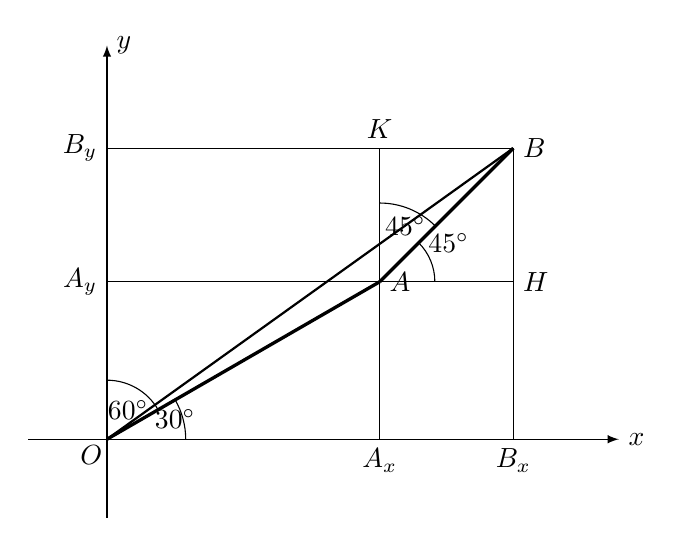
\begin{tikzpicture}[>=latex]
\draw[->](-1,0)--(6.5,0)node[right]{$x$};
\draw[->] (0,-1)--(0,5)node[right]{$y$};
\draw (2*1.732,0)node[below]{$A_x$}--(2*1.732, 2)node[right]{$A$}--(0,2)node[left]{$A_y$};
\draw (2*1.732+1.2*1.414,0)node[below]{$B_x$}--(2*1.732+1.2*1.414, 2)node[right]{$H$}--(2*1.732+1.2*1.414, 2+1.2*1.414)node[right]{$B$}--(2*1.732,2+1.2*1.414)node[above]{$K$}--(0,2+1.2*1.414)node[left]{$B_y$};
\node at (-.2,-.2){$O$};
\draw (2*1.732+1.2*1.414, 2) rectangle(2*1.732,2+1.2*1.414);

\draw[very thick] (0,0) -- (2*1.732, 2);
\draw[ thick] (0,0) -- (2*1.732+1.2*1.414, 2+1.2*1.414);
\draw[very thick] (2*1.732, 2) -- (2*1.732+1.2*1.414, 2+1.2*1.414);

\draw(1,0)  arc (0:30:1) node[below]{$30^{\circ}$};
\draw(0,.75) arc (90:30:.75)node[left]{$60^{\circ}$};
\draw (2*1.732+.7, 2) arc (0:45:.7) node[right]{$45^{\circ}$};
\draw (2*1.732, 3) arc (90:45:1) node[left]{$45^{\circ}$};


\end{tikzpicture}
